\section{Описание}

Поиск A* — в информатике и математике, алгоритм поиска по первому наилучшему совпадению на графе, который находит маршрут с наименьшей стоимостью от одной вершины (начальной) к другой (целевой, конечной).


Порядок обхода вершин определяется эвристической функцией «расстояние + стоимость» (обычно обозначаемой как f(x)). Эта функция — сумма двух других: функции стоимости достижения рассматриваемой вершины (x) из начальной (обычно обозначается как g(x) и может быть как эвристической, так и нет), и функции эвристической оценки расстояния от рассматриваемой вершины к конечной (обозначается как h(x)).


Функция h(x) должна быть допустимой эвристической оценкой, то есть не должна переоценивать расстояния к целевой вершине. Например, для задачи маршрутизации h(x) может представлять собой расстояние до цели по прямой линии, так как это физически наименьшее возможное расстояние между двумя точками.


Этот алгоритм был впервые описан в 1968 году Питером Хартом, Нильсом Нильсоном и Бертрамом Рафаэлем. Это по сути было расширение алгоритма Дейкстры, созданного в 1959 году. Новый алгоритм достигал более высокой производительности (по времени) с помощью эвристики. В их работе он упоминается как «алгоритм A». Но так как он вычисляет лучший маршрут для заданной эвристики, он был назван A*.


A* пошагово просматривает все пути, ведущие от начальной вершины в конечную, пока не найдёт минимальный. Как и все информированные алгоритмы поиска, он просматривает сначала те маршруты, которые «кажутся» ведущими к цели. От жадного алгоритма, который тоже является алгоритмом поиска по первому лучшему совпадению, его отличает то, что при выборе вершины он учитывает, помимо прочего, весь пройденный до неё путь. Составляющая g(x) — это стоимость пути от начальной вершины, а не от предыдущей, как в жадном алгоритме.


В начале работы просматриваются узлы, смежные с начальным; выбирается тот из них, который имеет минимальное значение f(x), после чего этот узел раскрывается. На каждом этапе алгоритм оперирует с множеством путей из начальной точки до всех ещё не раскрытых (листовых) вершин графа — множеством частных решений, — которое размещается в очереди с приоритетом. В моем случае был выбран массив или map. Приоритет пути определяется по значению f(x) = g(x) + h(x). Алгоритм продолжает свою работу до тех пор, пока значение f(x) целевой вершины не окажется меньшим, чем любое значение в очереди, либо пока всё дерево не будет просмотрено. Из множества решений выбирается решение с наименьшей стоимостью.


Множество просмотренных вершин хранится в closed, а требующие рассмотрения пути — в очереди с приоритетом open. Приоритет пути вычисляется с помощью функции f(x) внутри реализации очереди с приоритетом.

\section{Реализация на p5.js}

При реалиации алгоритма я начал с проектирования его на языке java script в библиотеке p5.js.

Я создал grid, в котором могу самостоятельно выставлять начальную и конечные точки, а также ставить препятствия, через которые невозможно пройти.

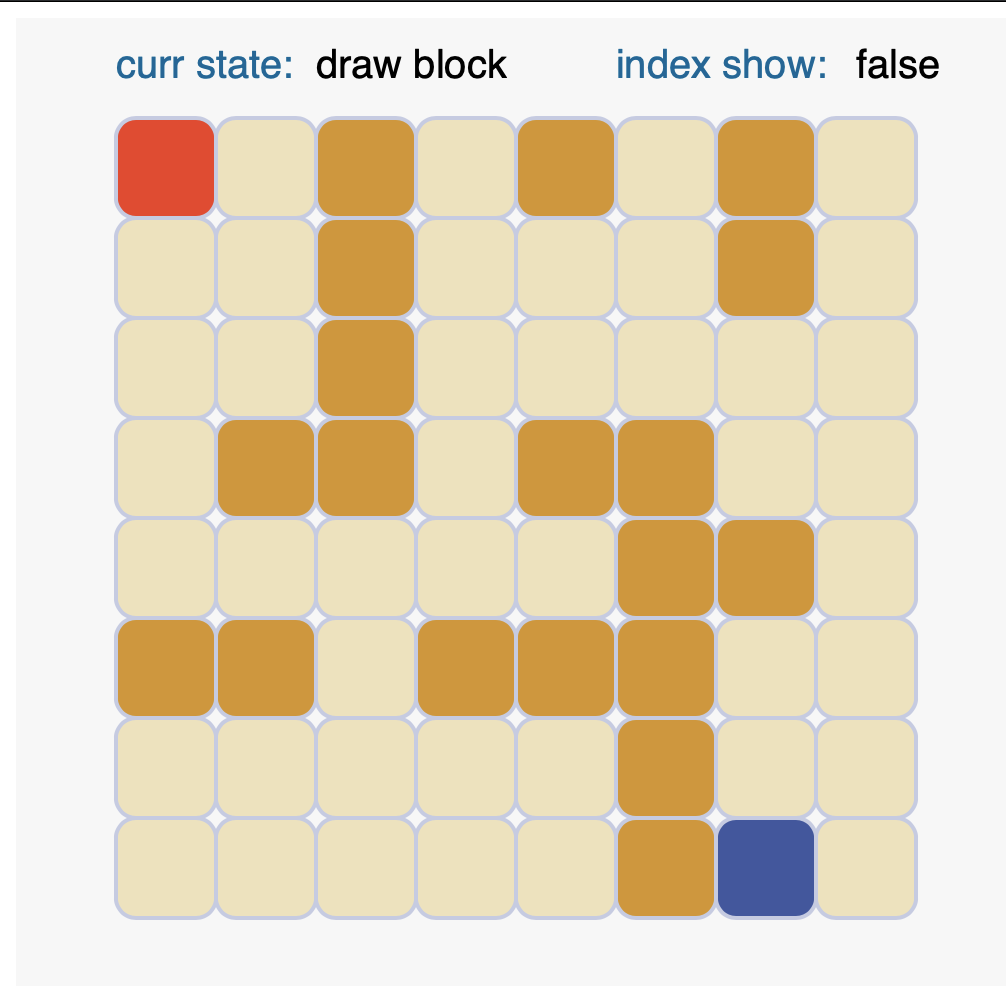
\includegraphics[scale=0.75]{pictures/1.png}

При нажатии клавиши F будет отображен путь в данной структуре.

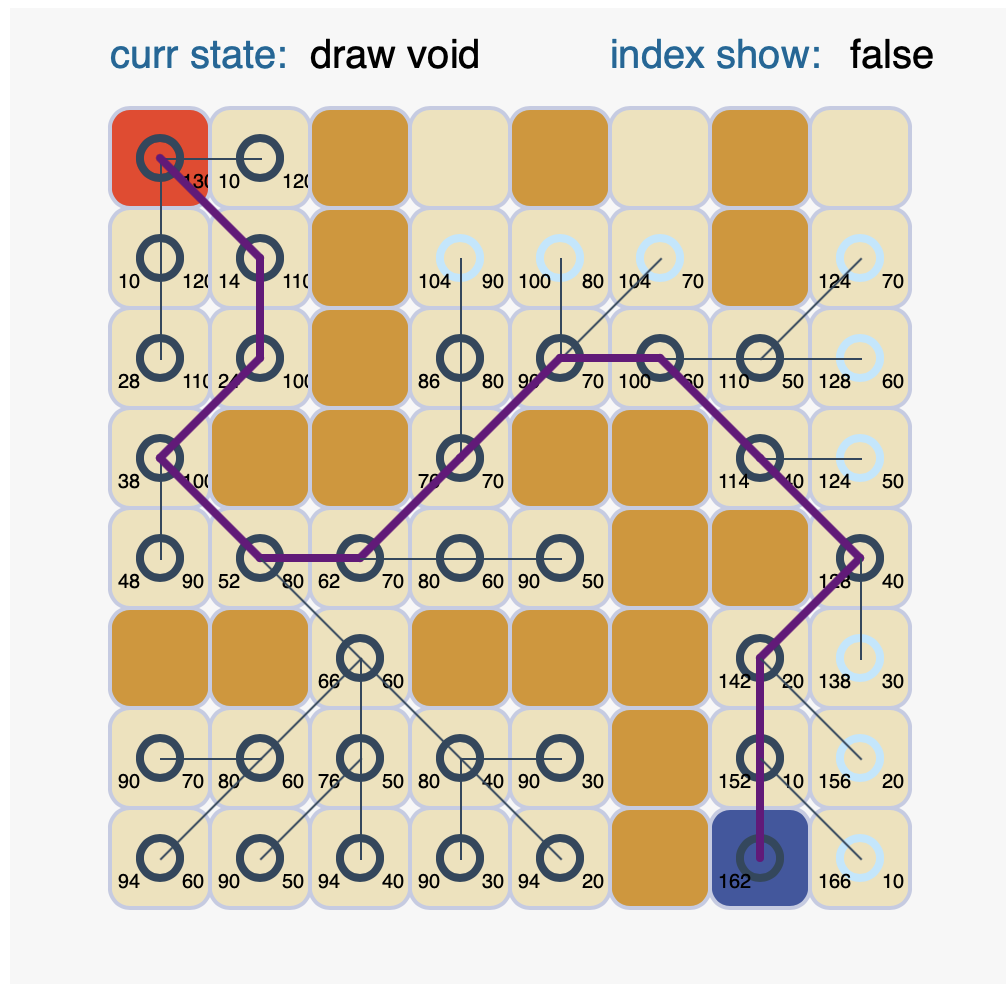
\includegraphics[scale=0.75]{pictures/2.png}

Алгоритм находит лучший путь в данном лабиринте на основании заданной эвристики. Отображает путь фиолетовой линией. Черные кружки отображают какие вершины уже просмотрены и находятся в closed, светлые, это те, которые находятся в очереди open. Также в каждой клетке слева внизу пишется расстояние до начала, для пути по диагонали оно составляет 14 единиц, а для прямого пути 10 единиц. Справа же пишется кол-во клеток до конечной вершины умноженной на 10. Такова выбранная эвристика.

Сразу можно увидеть недочет, вместо того чтобы пойти сразу вниз от старта, алгоритм сначала уходит вправо, что сразу дает неверный минимальный результат, но вспоминая, что алгоритм дает наилучший путь для заданой эвристики, можем утверждать, что эвристика, выбранная нами, не является оптимальной для данной задачи, так как не всегда дает минимальный возможный путь.

При нажатии клавишы p - программа выдает на скачивание серииализированный файл, который мы сможем скормить программе на С++, в которой реализованы сразу два алгоритма, А* и Алгоритм Дейкстры.

\pagebreak

\begin{lstlisting}[language=Javascript]
function A_star() {
	let open = [];
	var start = {i:points.start.i,j:points.start.j};
	var end = {i:points.end.i,j:points.end.j};
	open.push(board[start.i][start.j]); // color it like open blue circle
	board[start.i][start.j].open = true;
	board[start.i][start.j].d = 0;
	board[start.i][start.j].h = (abs(start.i - end.i) + abs(start.j - end.j)) * 10;
	while (open.length != 0) { // find closest open
		var min_el = null;
		var min_dist = 100**100;
		for (var i = 0; i < open.length; i++) {
			if (open[i].open && open[i].d + open[i].h < min_dist) {
				min_el = open[i];
				min_dist = open[i].d + open[i].h;
			}
		} // delete it // color it black circle
		var p_i = min_el.i;
		var p_j = min_el.j;
		board[p_i][p_j].open = false;
		board[p_i][p_j].closed = true; //if it is end then draw path
		if (p_i == end.i && p_j == end.j) { // draw big lines from end to start
			var p = min_el;
			while (p.parent != null) { //draw line
				p.main_parent = p.parent;
				p = p.parent;
			}
			return;
		} // for every child he have add them to open array // color them in blue circle
		var childs = find_close_cells(p_i, p_j);
		for (var i = 0; i < childs.length; i++) {
			open.push(board[childs[i].i][childs[i].j]);
			board[childs[i].i][childs[i].j].open = true;
			board[childs[i].i][childs[i].j].h = (abs(childs[i].i - end.i) + abs(childs[i].j - end.j)) * 10;
			var new_d = board[p_i][p_j].d;
			if (abs(childs[i].i - p_i) + abs(childs[i].j - p_j) == 2) { new_d += 14; } 
			else { new_d += 10; }
			if (board[childs[i].i][childs[i].j].parent == null) {
				board[childs[i].i][childs[i].j].parent = board[p_i][p_j];
				board[childs[i].i][childs[i].j].d = new_d;
			} else {
				if (board[childs[i].i][childs[i].j].d > new_d) {
					board[childs[i].i][childs[i].j].parent = board[p_i][p_j];
				}
			}
		}
	}
}
\end{lstlisting}

\pagebreak

\section{Реализация на C++}

Что касается кода на С++, то я создал структуру графа, по которой и будет происходит поиск пути, сам по себе алгоритм особо не меняется, для начала приведу код Дейкстры, чтобы сравнить в дальнейшем с А*.

Вот так выглядит сам граф, вектор вершин, в каждом из которых лежит хеш таблица ребер до других вершин. Само ребро является отдельной структурой со своим конструктором.

\begin{lstlisting}[language=C++]
private:
    struct Node;
    struct Edge {
        Edge() = default;
        Edge(Node * node, const int waight) : node(node), waight(waight) {}
        Node * node;
        int waight;
        ~Edge() = default;
    };
    struct Node {
        Node() : d(__INT_MAX__), h(__INT_MAX__), parent(-1), x(0), y(0) {}
        unordered_map <int, Edge> edges;
        int d;
        int h;
        int parent;
        int x, y;
        ~Node() = default;
    };
    int size;
    vector <Node> nodes;
\end{lstlisting}

\pagebreak

\section{Алгоритм Дейкстры}

В алгоритме Дейкстры мы не найдем использования переменной d, На каждом этапе мы просто достаем вершину из map open, для всех ее детей расчитываем новый минимальный путь, если он оказывается меньше чем уже имеющийся, мы меняем родителя у ребенка на нового, если нет, то оставляем все как есть. После обработки, выбранная вершина отправляется в массив closed, отмечается там как посещенная и больше никогда не рассматривается. Как только алгоритм дойдет до финальной вершины, он бросит все дела и начнет собирать результирующий массив, далее его переворачиавет и отправляет результатом.

\begin{lstlisting}[language=C++]
vector <int> Dijkstra(int from, int to) {
        vector <int> res;
        nodes[from].h = 0;
        map <int, Node *> q;
        pair <int, Node *> curr;
        vector <bool> visited(size, false);
        int min_curr;
        q[from] = &nodes[from];
        while (q.size() != 0) {
            min_curr = __INT_MAX__;
            // find minimum from open
            for (pair <int, Node *> elem : q) {
                if (elem.second->h < min_curr) {
                    curr = elem;
                    min_curr = elem.second->h;
                }
            }

            if (curr.first == to) {
                res.push_back(to);
                int p = curr.second->parent;
                while (p != -1) {
                    res.push_back(p);
                    p = nodes[p].parent;
                }
                break;
            }
            // for its child add them to open
            // remake childs h paremetr
            for (pair <int, Edge> child : curr.second->edges) {
                if (visited[child.first] != true) {
                    // add child to open q
                    q[child.first] = &nodes[child.first];
                    // if less h make new
                    int h_min = curr.second->h + curr.second->edges[child.first].waight;
                    if (h_min < nodes[child.first].h) {
                        nodes[child.first].h = h_min;
                        nodes[child.first].parent = curr.first;
                    }
                }
            }
            // delete curr from q
            q.erase(curr.first);
            visited[curr.first] = true;
        }
        if (res.size() != 0) {
            reverse(res.begin(), res.end());
        } else {
            res.push_back(-1);
        }
        return res;
    }
\end{lstlisting}


\pagebreak

\section{Алгоритм А*}

Главным отличием от предыдущего алгоритма - наличие еще одного парамера, помимо d, параметра h, который считает Декартово расстояние (Евклидова метрика) от рассматриваемой точки до конечной.

При сравнении эвристики на js и С++, данная эвристика дает чаще лучший результат, и не ходит там, где браузерная версия пошла бы.

На каждом этапе из map open берется элемент с минимальной $d + h$, после чего для всех его потомков проставляется число d и h, при необходимости обработки уже открытых элементов, алгоритм может изменить d, но никак не h, в том числе может изменить предка у вершины, если на данном этапе путь до этой вершины из активной меньше, чем уже имеющийся.

При организации очереди с приоритетом или кучи по $d + h$, можно было бы добиться логарефмической сложности поиска минимального элемента, но при использовании std map, поиск идет итеративно за линию, а удаление и вставка за логарифм.



\begin{lstlisting}[language=C++]
vector <int> aStar(int from, int to) {
        vector <int> res;
        vector <bool> visited(size, false);
        nodes[from].d = 0;
        nodes[from].h = (int)sqrt(pow(nodes[to].x - nodes[from].x, 2) + pow(nodes[to].y - nodes[from].y, 2));
        map <int, Node *> q;
        pair <int, Node *> curr;
        int min_curr;
        if (nodes[from].h != __INT_MAX__)
            q[from] = &nodes[from];
        while (q.size() != 0) {
            min_curr = __INT_MAX__; // find minimum from open q
            for (pair <int, Node *> elem : q) {
                int d_h_curr = elem.second->d + elem.second->h; // d + h of some in q
                if (d_h_curr < min_curr) {
                    curr = elem;
                    min_curr = d_h_curr; // new min d + h
                }
            }
            if (curr.first == to) {
                // cout << "hello!\n";
                res.push_back(to);
                int p = curr.second->parent;
                while (p != -1) {
                    res.push_back(p);
                    p = nodes[p].parent;
                }
                break;
            }
            // for its child add them to open
            // if h ==  max int we wont add it to open q !!!
            // remake childs d paremetr
            for (pair <int, Edge> child : curr.second->edges) {
                if (visited[child.first] != true) {
                    // add child to open q
                    Node * curr_child = child.second.node;
                    curr_child->h = (int)sqrt(pow(nodes[to].x - nodes[child.first].x, 2) + pow(nodes[to].y - nodes[child.first].y, 2));
                    if (curr_child->h != __INT_MAX__) {
                        q[child.first] = &nodes[child.first];
                    }
                    // if less d + h
                    if (curr_child->parent == -1) {
                        curr_child->parent = curr.first;
                        curr_child->d = child.second.waight + nodes[curr_child->parent].d;
                    } else {
                        if (curr_child->d > child.second.waight + nodes[curr.first].d) {
                            curr_child->parent = curr.first;
                            curr_child->d = child.second.waight + nodes[curr_child->parent].d;
                        }
                    }
                }
            }
            // delete curr from q
            q.erase(curr.first);
            visited[curr.first] = true;
        }
        if (res.size() != 0) {
            reverse(res.begin(), res.end());
        } else {
            res.push_back(-1);
        }
        return res;
    }
\end{lstlisting}

\lstset{language=[gnu] make}
\lstset{
   language=[gnu] make,
   keywordstyle=\color{teal}\textbf,
   stringstyle=\color{blue},
   identifierstyle=\itshape
}

\begin{lstlisting}
CC = g++
CCFLAGS = -std=c++11 -Wall -pedantic
###____###
cpp : main.cpp *.hpp ; $(CC) $(CCFLAGS) main.cpp -o solution
js : sketch.js *.js ; open -a Safari index.html
clean : ; rm solution
\end{lstlisting}

\pagebreak

\section{Консоль}

\begin{alltt}
MBP-Pavel:src pavelgamov make clean
rm solution
MBP-Pavel:src pavelgamov make
g++ -std=c++11 -Wall -pedantic main.cpp -o solution
MBP-Pavel:src pavelgamov ./solution < /Users/pavelgamov/Downloads/newFile.txt 
A star time: 0.000157		
31 46 61 76 91 106 121 136 137 138 153 167 181 195 209 223 237 250 264 277 262 248 
Dijkstra time : 0.000921		
31 45 59 73 87 101 115 129 143 157 171 185 200 215 230 245 260 275 262 248 
\end{alltt}

\pagebreak